\chapter{Lore}

The \textit{Dreamshard} system was designed to be rather polyvalent, and can fit a variety of settings. That being said, it was built with its own custom setting in mind: a late medieval, low-fantasy world, which I shall present in this appendix.

\paragraph{In brief...}

In the recent past, the Dreamshard Isles have been shaken by unexplained magical phenomena. This, combined with an increase in finding of rare artifacts from the fabled Voskari mages, has attracted much outsider interest. More recently, the situation culminated with a volcanic eruption on Faris Island, which Magisters suspect might not be entirely natural... 

This is compounded by an already unstable geopolitical background with expansion efforts by the Atheryn Empire and other nations, while powerful Magisters vie for influence. The IDC, a branch of the Empire, is trying to expand in the Dreamshards and assert its influence, but other polities do as well. 

The players\footnote{Note that in terms of capabilities, the Player Characters as described by the rules are already a fair measure above a good chunk of the general population, especially when it comes to magic.} are mandated by the governor of the Empire's portion of the Dreamshards, a man named Lucius Clarence, to investigate the situation. They secured a ride on a ship, and are headed for the city of Port-Darla, a major metropolis and headquarters of the IDC.

\textit{What will they find? And should it have remained in the shadows?}


\section{Map}

The known world consists of four major landmasses: first, the Dreamshard archipelago to the West, presented on Map \ref{map_1}. Second, the world's largest continent, home to the Eastern Realms and located in the center of most world maps; it is partially presented in Map \ref{map_2}. Two other major continents exits: one to the East of the Eastern Realms (ironically), and one to the south.


\begin{figure*}[ht!]
    \centering
    \resizebox{1\textwidth}{!}{
        %\includesvg{img/map/map.svg}
        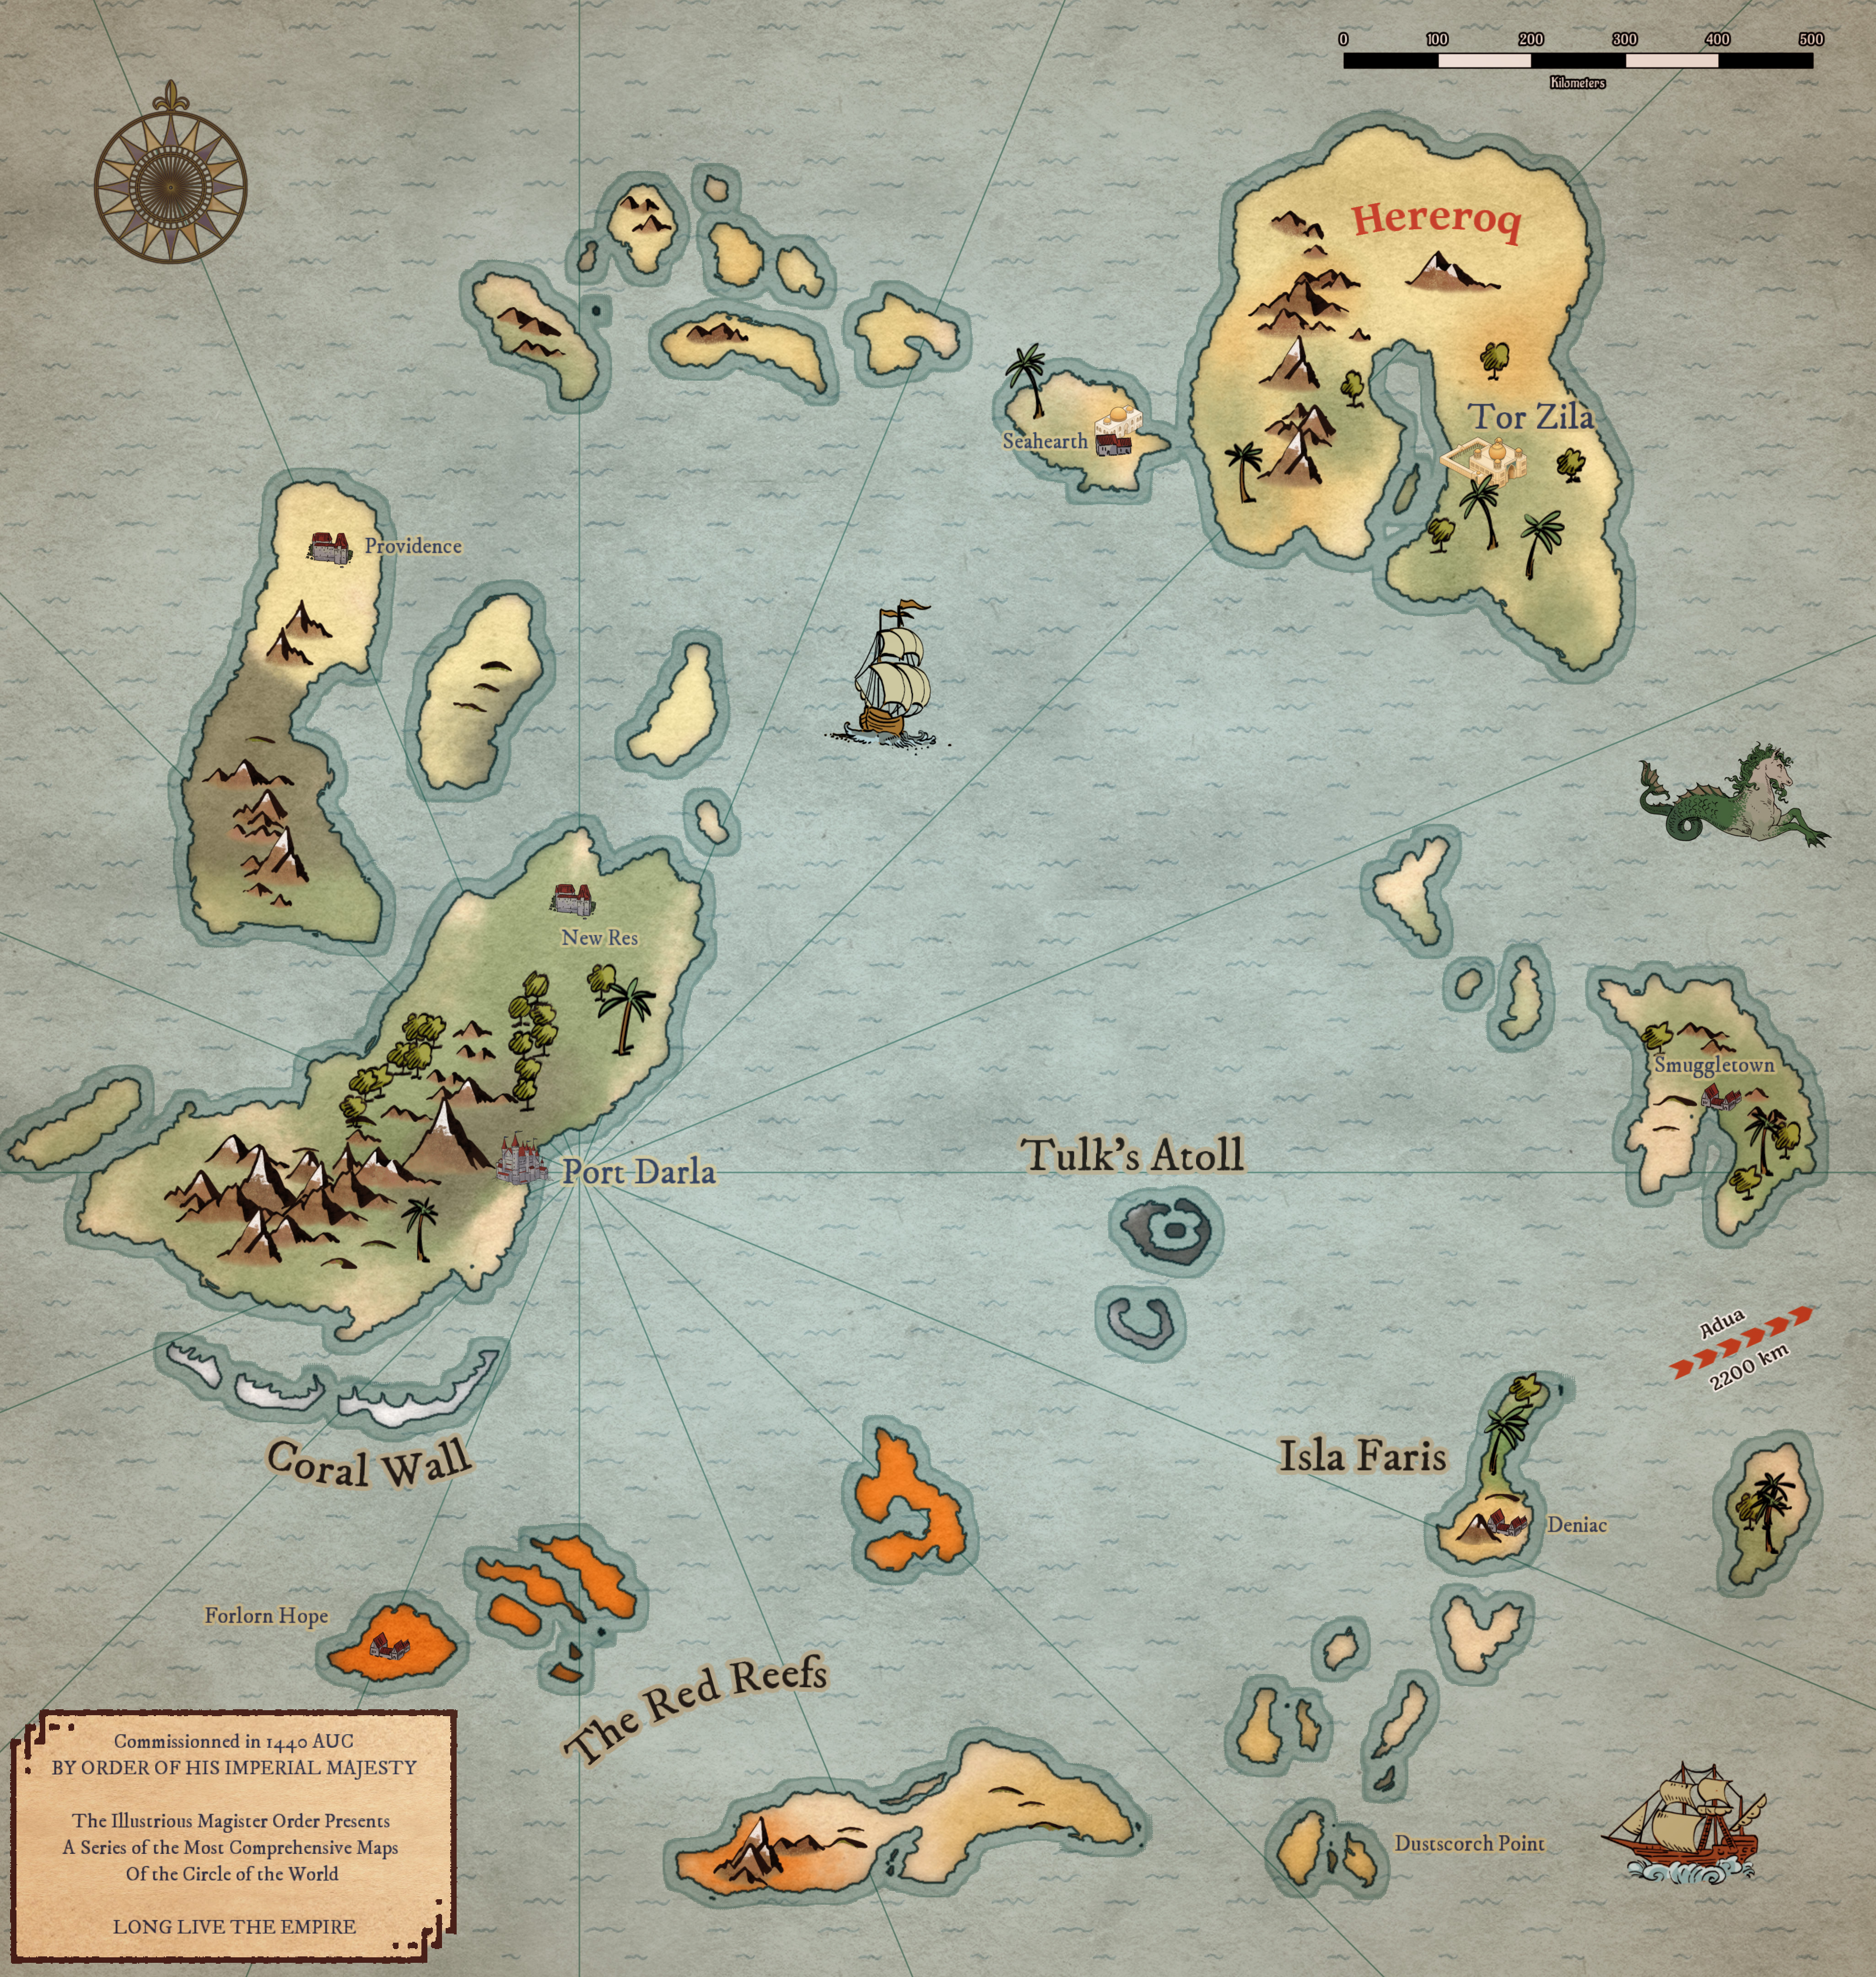
\includegraphics[angle=0,origin=c]{img/map_dreamshard.jpg}
    }
    \caption{Map of the Dreamshard Archipelago. Only major settlements are represented.}
    \label{map_1}
\end{figure*}


\begin{figure*}[ht!]
    \centering
    \resizebox{1\textwidth}{!}{
        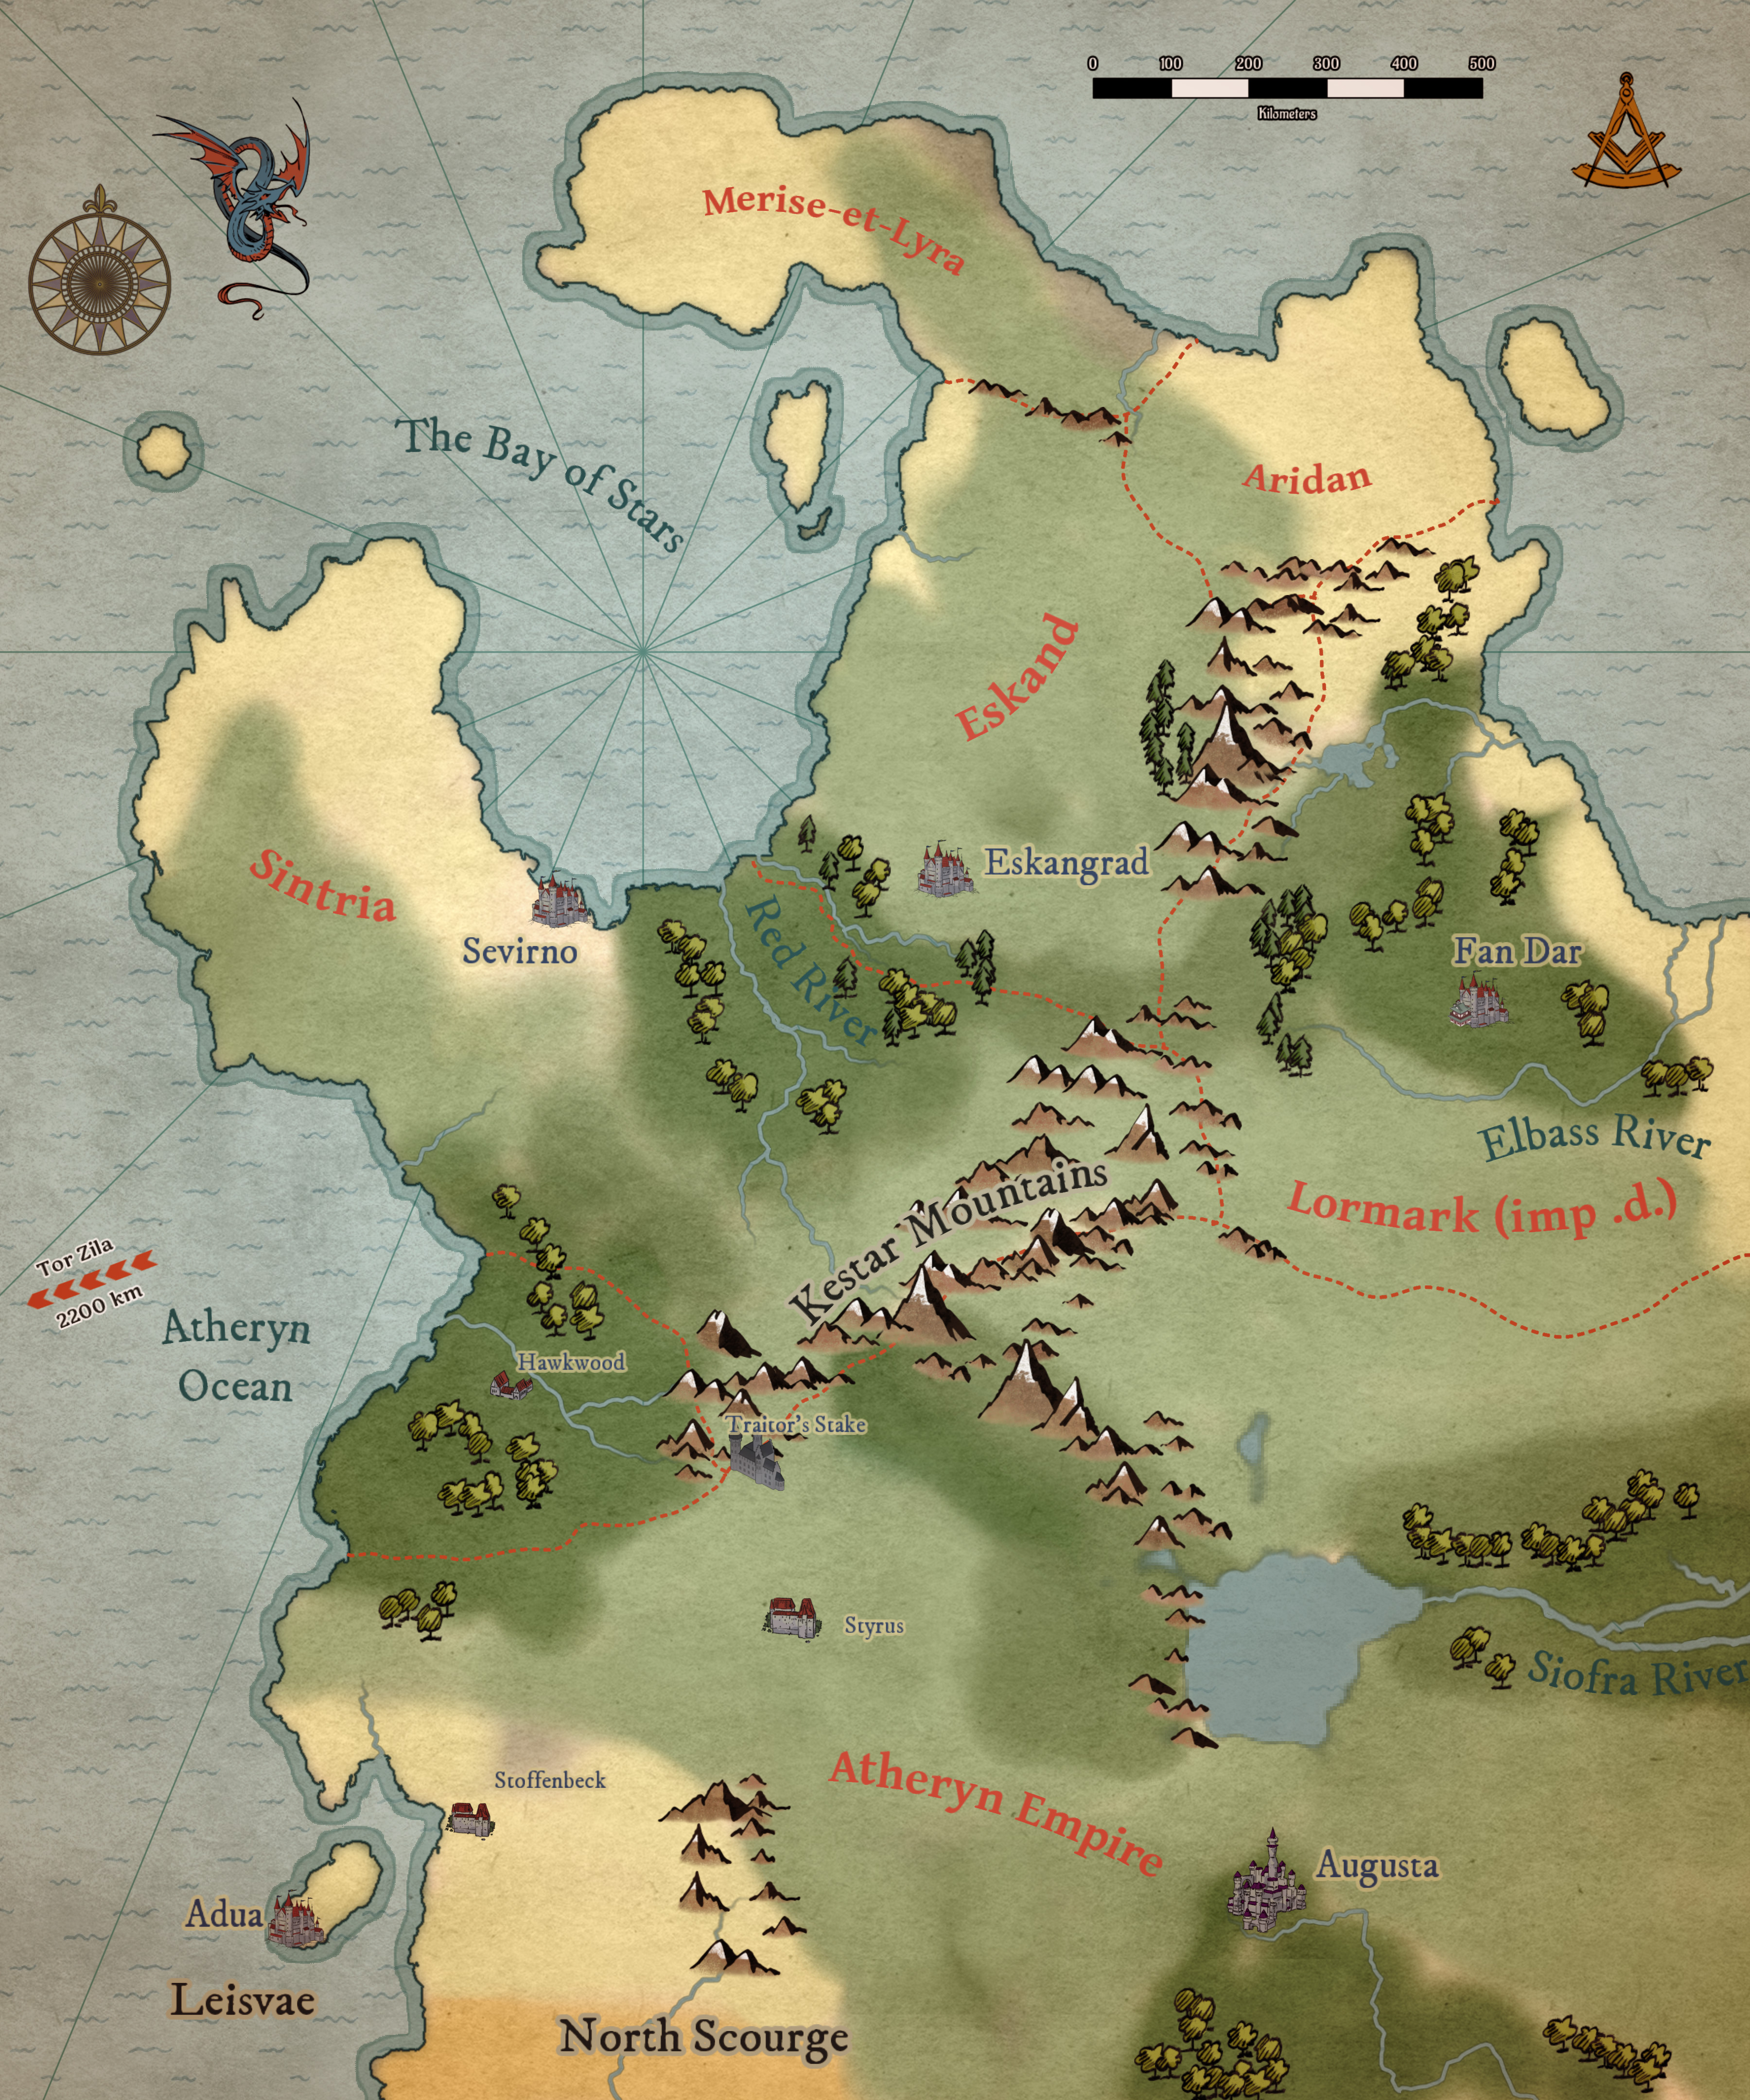
\includegraphics[angle=0,origin=c]{img/map_main_continent.jpg}
    }
    \caption{Map of the Eastern Realms, on the north of the Continent. Only major settlements and realms are represented. "Imp. d." stands for "Imperial dominion".}
    \label{map_2}
\end{figure*}




\subsection{Dreamshard Archipelago}

The Dreamshard Archipelago contains many large islands, some of which are contested. Its geography is presented on Map \ref{map_1}. It has a diameter of roughly 1800 kilometsrs, and its eastern edge is located about 2200 km from the western edge of the main Continent. As such, it can be reached in about two weeks.

Its largest island is home to Port Darla, its largest city. The northeastern large island is fully controlled by Hereroq. There are several smaller islands: Isla Faris to the southeast is warm and volcanic, and other landmarks include the island of Providence in the west.
       
Historically, the archipel has been settled for a long time. The latest wave of settlements (from the IDC, FSN, etc.) began only roughly a century and a half ago. They were mostly pursuing old \textit{de jure} territorial claims. Even so, the archipel remained a distant second fiddle in world affairs until an uptick in the rate of discovery of Voskari artifacts resulted in a regain of interest and thus a settlement rush, 75 years ago.

Owing to its size, the Dreamshard covers a breadth of latitudes, and as such it covers a gamut of virtually every climate. That being said, the most widespread biome is Mediterranean-like. Its south has a hot tropical climate, the middle has a warm climate with occasional dryness (especially in the southwest). But milder, temperate climates are found in the north, and the highest mountain chains have a cold climate.

The archipelago in rich in many important resources. Some are mainly commercial, like spices and olives. But the Isles are also also particularly rich in tellurium, a metal critical to industrial applications of Magic.



\subsubsection{Port Darla}

Port Darla is a boom town, and the headquarters of the Imperial Dreamshard Coumpany. It was founded by Francis Darla 62 years ago, with Lucius Clarence arriving as governor 4 years ago. 



\begin{rpg-quotebox}
    The advantage of having deep pockets? You can bury your foes in them. \\ \textendash \textit{Lucius Clarence}
    \end{rpg-quotebox}
    

It has become an important city of 30 thousand inhabitants, mostly funded by commerce incidental to the Dreamshard Rush. As a new city, it was built according to a geometric plan, with four main avenues corresponding to cardinal points.


\subsection{Eastern Realms}

The main continent, presented on Map \ref{map_2} is home to several polities. It is often referred by its inhabitants simply as "the Continent", capitalized, in an amusing display of chauvinism. Even just its northern part is large, with the distance between Sevirno and Augusta being roughly 1600 km in a straight line.

The most notable are the powerful Atheryn Empire, the independant Northern Kingdoms, and the semi-independant Lormark valley. It has a temperate cold climate to the north of the Kestar mountains, while the south has a warmer climate.

The extreme south and east of this continent (not depicted on the map) remain only partially explored by the aformentioned polities and are improprely called the "Uncharted Lands"\footnote{In concept, this is a blank canvas for players to propose any origin concept they want in accordance with the GM.}. This includes (but is not limited to) the Scourge, a dry steppe full of aggressive cultures, whic separates the so called Eastern Realms from other advanced civilisations on the two other continents, lengthening the required sea travel to meet them as there are fewer close ports.

\section{Cosmogony}

The planet is a sphere, has one moon called Sela, and orbits a yellow sun simply called "Sol". Known planets in the solar system include Lyria and Aulcus, and known constellations visible from the Dreamshard include the Chimera and the High Cross, which contains the Polar Star.

In the classical Atheryn Imperial calendar, used in the Northern Hemisphere, the year beging with spring and is divided in 12 months (Germinal, Bloomal, Landfall, Messidor, Sundary, Fructidor, Vendémiaire, Brumaire, Frimaire, Snowfall, Rainfall, Windfall) of 30 days each, plus an "out-of-calendar" week that celebrates the end of winter and the beginning of spring for this hemisphere. The first year of the calendar is the day of the founding of Augusta, the imperial capital. \textit{The current date is 18 Vendémiaire, 1440 A.U.C.}


\subsection{Magic}

\label{magic_lore}

Magic is a force that lets its practioners achieve all sorts of effects, some of which seemingly bend the laws of physics as we know them in the real world.

As best as anyone can tell, Magic seems a fundamental property of the universe. Humans are by far the best generators of magical energy: which is not surprising, since the prevailing theory is that magic is generated by sentience, as we will explain below.


\paragraph{Who can do it?}

Technically, everyone can perform Magic. In practice, however, wizards are an extreme rarity\footnote{About as frequent as champion athletes, virtuoso artists, PhDs, etc. are in the real world.}. This is because magic is extremely difficult, and has a poor cost-to-benefit ratio for most people: it takes the average person years to learn how to conjure a small flame, while even with primitive technology it takes only a few seconds to rub two flints together and make a fire. As such, for most people the investment is not worth it. Of course, like for literally anything else, some people will be naturally better at Magic. 


\begin{rpg-quotebox}
    "Power" is only defined in terms of who is able to stop you. \\ \textendash \textit{Who Said It}
\end{rpg-quotebox}

Indeed, for the more powerful, it's a different story. Those who can push past the break-even point are usually called "wizards", and the very best are called "Magisters". Magisters are extremely poweful, although not enough to call down meteors or perform similar cataclysmic events.

There exists a Magister Order which is meant, on paper, to be an association of those mighty few. But in practice, Magisters are almost completely autonomous. While there are Magic institutes teaching it in a traditional collegial manner, the rarity of skilled practicioners means most wizards learned through a more personal master-disciple relationship, with one master sometimes having several disciples, or simply by trial and error. Magic is studied scientifically by some, but remains very opaque. Tangentially, this explain the screwed-up formulation of prophecies and certain spells: they are written by trial and error, modifying them a word at a time to see what best matches the currents of Magic. 

This also means that, while people with temporal power (kings, etc.) are expected to have a basic understanding of Magic, few use it themselves\footnote{Like new technologies in the real world.}. Sorcerer Kings are often a terrifying prospect, and quite a few Emperors have been wizards. But since ruling can be a dangerous profession, most Magisters are content with acting as grey eminences to them instead of making plays to the throne themselves.

\paragraph{The nature of Magic} 

Magical potential is a combination of nature and nurture. Becoming a wizard is usually the result of dedicated study and practice, or in tangential cases of having enough money to throw at the problem. There is a puzzling exception to this rule: some people can have a instinctive affinity for Magic, which stems from a high Resolve, and from Greatness with a capital G. Intelligence helps understand and manipulate the Source of Magic in the general case, but strong wells of Magic can come from such Great People.

For instance, consider Saint Lucien, a prominent figure in the Dawning War, which is the founding event of the Atheryn Empire. He was as powerful as the best Magisters, if less adept at controlling his magic, and had only received minimal training. But he was known to be a charismatic leader and a very strong soul, and indeed his followers always seems to heal faster and survive wounds that should have killed them. It goes without saying that this fueled intense jealousy from the Magisters.

Relatedly, the beliefs of many people, even if they don't have individual Greatness, can still coalesce and have effects like the magic of an individual wizards, or even reinforce the magic of a Great Person. But in these cases, the effects are usually much more subtle. Gods do not actually exist, but this "clap your hands if you believe" effect means some people see Magic as a divine gift (some believe it is from the Voskari...) or an answer to prayer, or something akin to "unleashing one's inner potential".
	
These realizations led to the Source Theory: that Magic is power by \textit{sentience}. This is done consciously by Wizards, who use their Intelligence to channel Magic; not only the magic generated by their own sentience, but also to a lesser degree channel the general "magical field" that is present thanks to the mere existence of sentient beings. The rest of mankind can do this unconsciously, but much less efficiently. There is only one flaw in this theory, but it is a major one: it appears non-sentient animals, golems, and even a barren desert will have a small but nonzero level of Source present. In fact, the cosmos itself contains endless Magic, but with minute density. No satisfactory theory currently explains why.

Raw Magic can be stored in physical form. It's usually in this form that is it called "Source", unsurprisingly. Source behaves something like a gel, but consistently defies the laws of physics. However, it is not usable as-is and must be refined again through a Sigil to be effective.



\paragraph{How to use Magic}

Magic is performed through the proper Sigils, augmenting them with Accents to channel their power into a real-world effect. Each Sigil covers a certain type of effect, such as fire, healing, divination, to name a few.

The most common way to do so is by engraving or painting a Sigil on a support, but they can also be encoded in a vibration (music), for instance. Advanced inscribing will require special materials and tools. When casting a Spell directly, the Sigil is formed by hand movements, sometimes accompanied by vocal incantations. That being said, experienced wizards can be discrete and cast directly from their willpower, with no need for gestures or materials. This is, however, considerably more difficult. 

The main factors limiting the potential of Magic are intrinsic: gestures and engraving must be made with daunting precision to work, and they are extremely difficult to standadize, as the flow of Source is never exactly equal between two castings, even at the same position or at the same time. This means that the most common way to use Magic is to use Magical Implements prepared by wizards, which are consumable and cast a given spell.

Some forms of technology rely on Enchanting objects or machines to incorporate Magic into their working. This is rather rate, but gaining in popularity, to the point of kickstarting an industrial and scientific revolution recently. But this is costly: an enchanted object will cost many golden marks, and as such the practice is limited to specialized applications and only has noticeably impacted some high-value, high-technology industries.

Tangentially, even more potent Magic can be created by working at a more fundamental level through the Source Sigil. This is however enormously difficult and very finicky, and as such is not available to the players by default. It should be a "plot device" only if needed.

Based on Source Theory, it is also possible to Purge someone or something (not just humans, and indeed not just living things) to extract their Source and strengthen Magic, but this is obviously frowned upon by most. The Voskari refer to this as Expiation.


\paragraph{Effects and limitations}

\label{magic_effects}

While Magic can have many wondrous effects, its will remain fairly limited in scale. In particular, I would refer you to the description of the different Sigils, which is given in section \ref{abilities_list}, to get a general idea of what is possible. In this section, I will give additional clarifications.

In terms of scale, for instance, conjuring fireballs is extremely rare, and magical healing will usually be restricted to immediate knitting of the flesh and accelerating natural recovery. Bar the most powerful Magisters in history, nobody is powerful enough to call down meteors. On that note, only Magisters can acheive anything really spectacular: Magisters can extend their lives (but mostly only by decades, not centuries\footnote{Uber-powerful Magisters can end up befriending familiy lines instead of individuals, justifying it as "it's just like befriending a person, but dezoomed. You befriend the ones you like, and sometime people change, just like families"}).

Divination is possible, but they are in fact a form of predictive algorithms that tap into the subconscious computing power of the caster's mind. It may also be used to talk to animals, or in other languages. Also used for remote communications, but long distance is difficult so reserved for strategic commmunications and done by magisters only.

Sigils such as Nature or Summoning may be used for limited  metamorphosis and mutagenic purposes, but manifestations of Summoning are very impermanent. -> Conjuration of physical matter out of nothing is going to be EXTREMELY limited. 

It is also possible to be creative: for example Telluric and Force have many engineering applications.

While many powerful effects like space-time manipulation and even creating new planes of existence creation (!) are theretically possible with the Source Sigil, the immense amounts of power required are out of reach. For the moment, at least...
 \footnote{For the lulz, remember that source sigil can fuck up with time and fundamental laws of the universe. Like hossenfelder said, left to right backwards in time = right to left forward so (I) note the actions that have been performed and in which order, like chess notation, so you may cancel them. Also "bending time and space" in general, which can be warp drive or wormhole or ark or whatever}



\paragraph{Echos}

Echos are remnants of people, a magical fac-simile created by the residual impact of their sentience. They manifest as ghosts, but are very unstable and nowhere near as smart as the alive person. When someone is still alive, their Echo does not manifest as it is (usually....) drowned out by their full personality, much like the wave of a pebble thrown into the sea is erased by a tsunami. 

However, the greater resolve the person had in life, and the better they were at magic, the stronger the Echo. These effects are cumulative, hence not just Magisters can become those, people with great Resolve too. They can also be manually made by "infusing" pople with magic, but this is failure-prone.


\begin{rpg-quotebox}
    From across time and space, they will answer the call. \\ \textendash \textit{Merivahn}
\end{rpg-quotebox}
     
Echos can be an impactful force and have effects in the 'real' world (ie. poltergeists). Echos are broadcasts and do not necessarily require a body to last.
    
Echo manipulation views differs. Generally people have a favorable view of magic (mainly Atheyn Empire and Lormark) will view it more favorably. Others will be split between awe, wonder, and wariness.

\footnote{Some random echos found by accident in the aetheral suggest the existence of other sapient species far away, perhaps on another plane. At least some are from our Earth.}


\subsection{Bestiary}


\rpgart{t}{img/art/kelp}

The only naturally sapient race are Humans. Other sentients beings are so rare as to be anecdotal, and it should be notes that all of them are either magical creations or "meta-humans" (humans altered by magic)
\footnote{Genes can be selected for, creating specific family lines, epigenomics nonwitstanding. Indeed, Magisters are particulary adept at eugenics.}. \footnote{Artificial sapients are limited by the same biological constraints (brain maturation, etc.) and owing to brute force/ trial and error/ artisanal  nature of their creation often have very unstable genomes (in the sense of containing many deleterious mutations and sometimes uneven numbers of chromosomes), so are usually sterile or breed slower than even humans ; clin d'oeil : some Magisters even manufactured anthropomorphic human-animal hybrids for... sordid purposes.}

On the flip side, this means that someone determined enough can create whatever screwed-up monstrosity they wish, sentient or not. But creating something that can be perennous in an ecosystem requires great power and great knowledge, so these remain rare and anecdotal. They are often a byproduct of voskari or mad magister experiment and can act as Source reserve vats for them. As such, all "monsters" possess a craving for Source (ie. unrefined Magic).



\paragraph{Synths}





All magically-made creatures are called Synthetics. This includes whole-cloth artificial creatures like above or heavily mutated ones, but creature evolution can be influenced by Magisters in a more subtle manner.


As the voskari fallout attests, ambient magic being released can have this effect, introducing controlled or uncontrolles mutations \footnote{While natural evolution takes millenia, although microevolution of small characteristics can be done over a few generations (depending on generational speed)
\footnote{Quadrupeds will generally share a bone structure and muscle attachments, traces of which can be seen in fish even. Muscle attachments for the face are cheekbones and lower far mandible} (although scapula have different angles and first joint is closer to body, also share muzzle extrusion but with differing shapes ofc), beyond that chordata. Magic can be used to SPEED ALL OF THIS UP CONSIDERABLY.}


\paragraph{Synth construcs}

An important other aspect is the existence of constructs, aka. golem and robots animated by magic, which are also technically "Synths". They can be partially organic or sometimes even fully inorganic. While those remain difficult to manufacture and hence rarely use, they are efficient calculators and can sometimes have some modest level of sentience. As such, those constructs are used to analyse large amounts of data and to perform hard labor. A philosphical dilemma is currently brewing on what moral status they should have.

Two other dilemmas : they are improving quicky and could conceivabley become fully sentient. As such, could they become wizards ? It is argued that their brand of sentience bears significant differences to humans' and they are not focused on imitating humans but on high level mathematics, so this is uncertain. This is mere speculation. For now, at least...







\subsubsection{Creatures}


There are some natural species however that do not exist IRL, such as the shuddaka trees and those weird horses, but they are rare.




Among the menagerie


- Arachnoid experiment
- Animated trees
- Animated armor/Golem
- Drillworm?
- Bone Bishop
- Occult reanimation specialist
- Drake purger
- Bismuth/tellurium golem
- Enthralling fungus
- Drowned ones
- Ashmen
- Kraken
- Hereroq windcaller
- Ghosts/echos
- "Demons" which are the result of Voskari experiments:	MANY, MANY fucked up Giger-esque Voskari-created monstrosities (ashmen included, and giger-esque machine tyrants) –> mentioned as "rumors"
- Constructs : golems, replicas
- Avatars: lupine anger, or avatars of strong emotions, works a bit like chaos demons in Warhammer 40k, and are close to Echos in their principle.





- Elephants and camels somewhere, in addition to cavalry (off handedly mention all three species being indigenous to Dreamshard, albeit in different biomes)
- Put in some dinosaurs in a lost island ! (conserved magically ?) they also conveniently explain some "monstrous" creatures, just like IRL !

- A few ideas: at least some those (though likely created by Magisters) have an ecological niche and are not synthetics
	trees with blue leaves and silver trunk, caused by the presence of actual silver, with communicating roots
	giant pillars-like coral formations
	coastal algae srpouting into the air thanks to air balloons
	monkey with a collar of sort of tentalcles for better prehension
	horses with boney crest for muscle attachment for additional strength
	large (mammoth-sized) animals with a flock of supporting organisms, killfish style
	basaltic organs are a must have! Idea: have some gradually slit tout, like missiles launching, and then explode in the air
	catlike species with very elastic tendons, can bend its spine into nighmarish contortions
	bird with mirror-like scales (yeah... I know) it can rotate while flying to reflect light or distract predactors
... as for size show a little of everything. i don't think i will go all the way up to something like massive dinosaurs, maybe one or two representants of almost extinct species, or an Abomination.



Off handedly mention that many of them can map to existing Bestiary profiles with only minor adjustments



\section{People and Cultures}

The world contains a variety of peoples and cultures, organized in a breadth of nations and polities.

The Eastern Realms, which designated the nations of the central Continent including the Atheryn Empire, have launched quasi-colonial enterprises to the Dreamshard Archipelago as a reaction to recent events. This, understandably, made the local potentates wary and had led to a sequence of portentous events (see section \ref{recent_history}).






- Describe skin tone and physical appearance of the peoples. Hereroq should be brown, lormark a bit more east-asian-ish but with high diversity, empire is mediterranean, north is european, find a bit more (notably there are blacks far to the south in a southern continent beyond the sand scourge, much like there is likely an eastern continent with asian-ish and brown-ish people



\subsection{Factions and History}

Flags in Figure \ref{flags}.

\begin{figure}[!ht]
    \centering      
        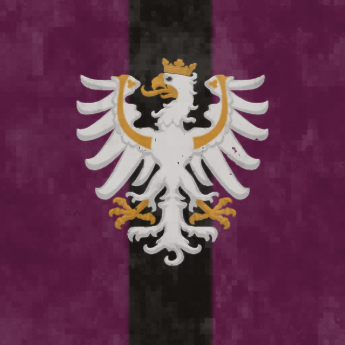
\includegraphics[scale=0.25]{img/flag/atheryn.png}
        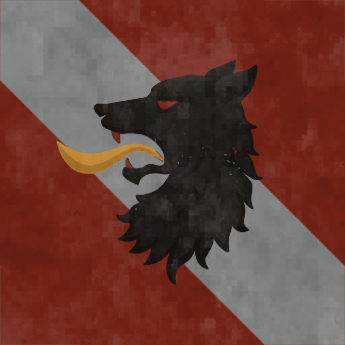
\includegraphics[scale=0.25]{img/flag/eskand.png}
        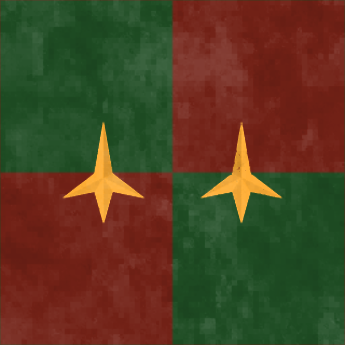
\includegraphics[scale=0.25]{img/flag/fnc.png}
        
\includegraphics[scale=0.25]{img/flag/fsn.png}
        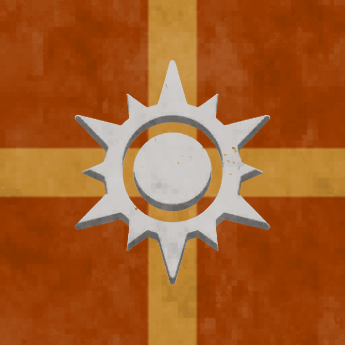
\includegraphics[scale=0.25]{img/flag/hereroq.png}
        
\includegraphics[scale=0.25]{img/flag/idc.png}
        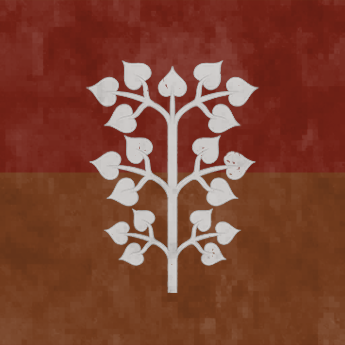
\includegraphics[scale=0.25]{img/flag/locals.png}
        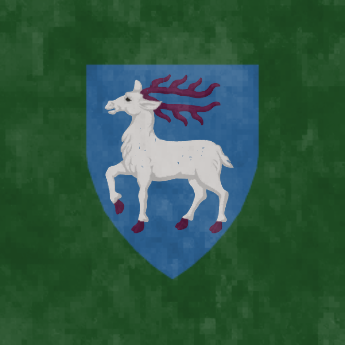
\includegraphics[scale=0.25]{img/flag/lormark.png}
        
\includegraphics[scale=0.25]{img/flag/sintria.png}
        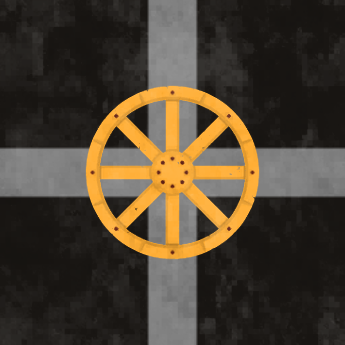
\includegraphics[scale=0.25]{img/flag/voskari.png}

    \caption{Flags of respectively, in classical reading order (left to right on each successive line, moving in lines from top to bottom): the Atheryn Empire, Eskand, the First Northern Company, the Free Sailors Nation, Hereroq, the Imperial Dreamshard Company, the local Dreamshard dukedoms, Lormark, Sintria, the Voskari.}
    \label{flags}
\end{figure}



\subsubsection{Atheryn Empire}


A powerful empire ruling over the central part of the Main continent. Southern European/Spanish/Byzantine culture. 


\textit{Leader}: Emperor Varen Atheryn the First.

\textit{Population}: estimated 40-60 million inhabitants (50-70+ with dependencies)

\textit{Wealth per capita}: Moderate on average, but with significant inequalities: presence of a very rich elite class, and a considerable poor underclass. For dominions and dependencies, it is very variable.

\textit{Territory}: Most of the center of the Continent, with its capital at Augusta
    
\textit{Colors}: Purple (major), white and black


\begin{rpg-quotebox}
Quote \\ \textendash \textit{Source}
\end{rpg-quotebox}


Founded by Saint Lucien in the Dawning War (see above)

More old-school antique (read: roman) ideas of empire. Very much believe in their civilizing mission: not quite racist, but very culture-supremecist, and believe they should spread the benefits of Empire far and wide and send many colonists. They embrace locals converts and syncretism, as long as the resulting mix is more Atheryn. However, defiance and refusal are met with brutal repression. 

Architecture is neo-classical

Politics are very backstabby, and although there are Families, individuals can rise, Caesar or Octavian style. There IS A SENATE, Roman style, but senatorial mandates are VERY long and suffrage is restricted to imperial citizens (but since Atheryn culture believes in its universalists pricniples, there is a path to citizenship) so elections are not as important as, say, today IRL, or even the true ancient rome. This makes it more meritocratic, as titles are not necessarily hereditary (in practice, Families are a thing, and heirs offten carry on, but nominally it's antique imperial system. Les grandes familles sont à couteaux tirés, et se disputent le contrôlent du Sénat. The Empire's great family often use special covert operatives against each other and exterior threats 

They are very sensible to Magister-like politics, and Magisters are often the cornerstones of the great families. Current Emperor, Varen Atheryn, is a very skilled Magister. Apocrypha : university at Augusta, capital of the empire. While the Empire is very scientistic (not a misspelling, I mean they are attached to sciene) there is a not-insignificant part of the pop that sees the Voskari as demigods and worships them, causing some internal tensions.
Note that the Empire is very bureaucratic. 

The Empire's fortunes have waxed and waned over the past millenia : it is currently closer to the Byzantine Empire than to the full glory roman empire. The northern kingdoms of Sintria and Eskand broke off a good century or two ago. The Atheryn empire has recently suffered a rather large civil war, Vakir's rebellion (Vakir was Sintrian in origin) Now that Varen Atheryn has ramassé les dents of the Empire, it looks outwards again.  no internal wars in the empire now since it's done ramasser ses dents. See recent evets. Some famous regiments include 1st 'Black Cross', 7th 'Devil's Heart' and the 11th 'Chimera'


The empire is the largest nation in the world and regroups a good 25-30 percent of world pop\footnote{Of the entire planet. If considering only the parts of the world it knows about, the empire's share of pop is larger.} However, not all that population has the same culture. The Atheryn heatlands have exported the Atheryn language, administration, and a bit of their culture, but syncretism remains the order of the day in the empire, and ensures its relative stability. 

The Empire has vassal states and duchies with tenuous control, such as Lormark, or Leisvae island, a major commercial and tellurium mining centre, recently suffering an attempted invasion by Eskand. (<-- this is mimbraine's imperial name, tell it to flo)

It should be noted that most of the Dreamshard is a \textit{de jure} part of the Empire, owing to early expeditions and treaties that are now centuries old, but it had attracted little interest and the locals were left to their own devices. Until now.



\paragraph{Imperial Dreamshard Company}

Short summary.

\textit{Leader}: Governor Lucius Clarence (it's complicated...)

\textit{Population}: 20K employees + 1.2 million Eastern colonists growing fast, plus a few million locals in the administered territories

\textit{Wealth per capita}: Moderate, but quickly improving.

\textit{Territory}: Port Darla and many isles

\textit{Colors}: Blue (major) and white (minor)


\begin{rpg-quotebox}
    "We shall bring civilization. Through the end of a musket, if need be."
    \end{rpg-quotebox}
    



The IDC is a dominion of the Atheryn Empire, of which most of the Dremshard Isles are a *de jure* part. They are resolutely expansionist, and use their large fleet to assert their influence in the archipelago. They also take an active interest in the magical phenomena affecting the archipelago.


The Imperial Dreamshard Company and FNC below are not simply extensions of their parent countries, they have some autonomy and disagreements with the mainland



\subsubsection{Northern Kingdoms}

The two main Northern Realms are Eskand and Sintria. There are a handful of other smaller ones (see the map), but they are almost all in the sphere of influence of the big two. Usually Feudal, with heredity of titles, and a pyramid of nobles and no suffrage.

\paragraph{Eskand}


Short summary.


\textit{Leader}: King Casamir (formerly), Lady Valskaya

\textit{Population}: 6 million (uncertain due to recent troubles)

\textit{Wealth per capita}: Low, partly due to recent troubles.

\textit{Territory}: a
    
\textit{Colors}: Red (major), white and black


\begin{rpg-quotebox}
Quote \\ \textendash \textit{Source}
\end{rpg-quotebox}



Used to be a junior partner in a personal union with Sintria under King Casamir II.
Broke free and has been in an uneasy peace with them, dotted with small wars.
    

Architecture would be best described as brick gothic



Sofia ?



\paragraph{Sintria}

Short summary.

\textit{Leader}: Leto III Seinfeld

\textit{Population}: 11 million

\textit{Wealth per capita}: Moderate.

\textit{Territory}: a
    
\textit{Colors}: Yellow and white


\begin{rpg-quotebox}
    Quote \\ \textendash \textit{Source}
    \end{rpg-quotebox}


Cultural offshoot of the Atheryn, was a province three centuries ago but now independant. Some, but not much, hard feelings as a result.

Architecture would be best described as modernized romanesque (renaissance)

Vakir (from the last imperial civil war) was Sintrian, hence tensions.

They have been expansionnist, lately.


Leto ?



\paragraph{First Northern Company}


Short summary.

\textit{Leader}: Director Alaria

\textit{Population}: approx. 15K employees + 750K colonists, growing, plus the locals in the administered territories

\textit{Wealth per capita}: High.

\textit{Territory}: Providence
    
\textit{Colors}: Red and green


\begin{rpg-quotebox}
"Enriching mankind and enriching oneself are not mutually exclusive goals."
\end{rpg-quotebox}


In the Dreamshard. Sponsored by Sintria and Eskand mainly, but also significant participation from merchants from Lormark (see below).  
The FRC is not simply extensions of their parent countries, they have some autonomy and disagreements with the mainland


They seek Profit, profit, and perhaps even more profit. Relatedly, there are averse to interventionism and military adventurism ; their philosophy instead centers around establihsing trading posts as opposed to very large scale settlements.

Several Houses vie for control of company interests.



\subsubsection{Lormark}

Short summary.

\textit{Leader}: Confederacy of city-states

\textit{Population}: 9 million, wealthier than average

\textit{Wealth per capita}: High, significant bourgeoisie.

\textit{Territory}: a
    
\textit{Colors}: Green and blue


\begin{rpg-quotebox}
Quote \\ \textendash \textit{Source}
\end{rpg-quotebox}

On paper, the Lormarkian principalties are grouped together as the Dominion of Lormark, which is a vassal of the Atheryn empire. However, the Empire takes a pretty lax approach and leaves them much autonomy, as long as they pay their taxes. Sometimes, they even remain in practice neutral in some imperial wars (although they join on paper)

Commerce focused

culture is a mix of east-asian-ish influence, with another sector being closer to india, have that reflected in their architecture by mentioning pagodas and stupas. In any case, VERY cosmopolitan, and heavily influenced (founded ?) by foreigners. Due to being founded by settlers and merchant foreigners from the most eastern continent (and a few from the southern) and hybridizig with local cultures

lormark should be a semi-unified kingdom-province (ie. few internal wars but not much beyond that), 

The current emperor (Varen) is seeking to turn them into a puppet state with tighter control, which is not sitting well with them.

	

\subsubsection{Voskari}

Short summary.


\textit{Leader}: Arch Lector Merivahn, supposedly

\textit{Population}: Unknown. Likely select.

\textit{Wealth per capita}: Unknown. Likely spectacular.

\textit{Territory}: Unknown
    
\textit{Colors}: Black (major) and yellow






\begin{rpg-quotebox}
	"Is gratitude still germane when directed at the wrong person ?"
\end{rpg-quotebox}

A riddle wrapped in a mystery. They share the Atheryn alphabet, but have their own language. Recognizable 19th-century stylistic elements mark them. Only few artifiacts of them have been found, but findings are accelerating. Artifacts belong to them are, like, 10-20 years ahead of the current technological level (not fantastically ahead, but quite advanced). The odd part is that this 10-20 years tech gap has remained constant ever since findings have begun, leading to speculation that they are still active and not an extinct civilization or an extinct Magister branch, and that they continue improving. Indeed, Some speculated to be an ancestor or branch to the Magister Order, with secret influence on the world. Speculated also to be behind many weird magical phenomena recently observed. One recurrent name : Merivahn.

they ARE homo sapiens, not aliens, and the tech is magic based so the other ones can catch up.
	
Worshipped as mythical demi-gods in certain places. In fact The voskari religion (meaning cult that worships voskaris) is quite organized, which can generate religious tensions. They believe the leftover Voskari artifacts are "gifts" to mankind, to put us "on the right path". 

In truth, they are pretty much the Illuminati cliché, interacting with the world, advancing science, and manipulating politics, but remaining as hidden as possible. It is important to note that they are far more than just a magic society. In fact, their focus on magic is simply a consequence of the fact that magic is one of mankind's most effective tools. They are a world-domination Illuminati-ish secret society first and foremost.
    Note that there are two subfactions : the White and the Reds. They have competing visions for the future, and this War in Heaven is a heavy plot points. The exact nature of these competing visions is left for the reader-GM to decide.

If you buy into the most common theories, and according to some anecdotal evidence, external recruitment is possible from outside the organisation even though inside recruitment is preferred, and the total number of voskari magister is rather limited to ensure few defections (they communicate magically). Defections from the Voskari have happened, but the Voskari disinformation game is strong so people don't generally believe them over their own pet theory (Voskari are gods, voskari are indeed magisters, etc.). The only tangible facts are the artifacts that share a common style and language. Those are the leaks that always happen since no conspiracy is ever foolproof.





\subsubsection{Hereroq}


Short summary.


\textit{Leader}: Archduchess (closest corresponding title in Atheryn language) Hesria

\textit{Population}: estimated 16 million

\textit{Wealth per capita}: Low, but slowly improving.

\textit{Territory}: Tor Zila, Seahearth, all Isle of Hereroq and dependencies
    
\textit{Colors}: Beige and orange


\begin{rpg-quotebox}
    "When the winds are changing, one must steer or die." \\ \textendash \textit{Hesria}
    \end{rpg-quotebox}


The native inhabitants of the Northern Dreamshard. While they shake hands with the Companies for now, the peace is tense and the Companies' outposts, including some of which are in Hereroq's dependencies, make the situation uneasy.


They are slightly backwards technologically compared to the Eastern Realms, but only slightly. Instead, their worst weakness is that they lack the wealth of the Companies, which are attempting to extract concessions, buy shares in their economy, make "unequal treaties", ... and conquer what they cannot buy. They will need to play their cards rights in the coming storm. 

use some Moorish architecture too. mix of Turkic, Moorish and Mesoamerican features, with pyramids and large roof overhands (don't say ottoman and meso, say things like ("pointed arches for doors and columns, domes maybe (but many small domes instead of big ones, to be distinct), sandstone-ish, describe wiki architecture, and mayan-style pyramids with incan-style blocks))"

Notables are named the Sifs, which are member of un upper social class that is starting to diverge from the rest of the people. Politically, this is an Union of cities: They are quite decentralized, with the Sifs ruling local. Queen Hesria is looking to centralize more and reform to stand against the other Great Powers. Membership to the Sifs' social class is inherited, though, but it is reasonably frequent for rich or influential people to be named Sifs by the queen or by prominent Sifs. Also, culturally there is a 'right to rebellion', and for certain positions they have suffrage but it is censitaire. This means their values are somewhat meritocratic, but their social structure makes them quite traditionalistic and reactionary, and political corruption is a problem.

Religion is important (though the voskari cult is proportionally less important here than in the Eastern Realms, local traditions keep a better foothold), and self-sacrifice as well is a national virtue. Anecdote : they have a few temples with wings that are periodically rebuilt facing another direction, to symbolize the passing of time.

Strong tradition of naval exploration (they initiated contact with the main continent way back when, not the other way around) but don't really care for expansionnism, their last outposts have been taken over, first by the local dukedoms decades ago, and now by company encroachment (both by buying out, simply resettling them, and a few low-intensity wars). Trading posts of theirs, however, remain throughout the Dreamshard, and a handful on the Eastern continent. Importantly, they have a reputation for spycraft / being excellent spies.


\subsubsection{Free Sailors Nation}

Short summary.

\textit{Leader}: "Admiral" Veraume

\textit{Population}: approx. 10K sailors, + locals

\textit{Wealth per capita}: Moderate, but only in fungible and not productive assets.

\textit{Territory}: Smuggletown
    
\textit{Colors}: Green (major) and teal

\begin{rpg-quotebox}
    "Let the empires bicker. We'll be there, quietly waiting to bleed them dry." \\ \textendash \textit{Source}
\end{rpg-quotebox}


Pirates operating almost exclusively in the Dreamshard. Sometimes, some among their numbers sell their services as privateers. Some Asian-ish elements (junks, came as some early leaders were fleeing from the asian-ish lands and brought those ideas, and catamarans from ancient natives for scouting and messages) but very patchwork. 

	
Your garden-variety pirate nation, loyal to no one but themselves, seeking profit above all else. Open to taking privateer jobs. They are not, however, bloodthirsty thugs, but attempts to form an organized nation have been met with defiance from within.






\subsubsection{Local Dreamshard petty realms}


Short summary

\textit{Leader}: Various

\textit{Population}: Unknown, estimated at a few million in total across the archipelago

\textit{Wealth per capita}: Low.

\textit{Territory}: a
    
\textit{Colors}: a

\begin{rpg-quotebox}
    Sleepless nights are very good at reminding you about all you have to lose. \\ \textendash \textit{Who Said It}
\end{rpg-quotebox}

Besides the great powers, there are local dukedoms native to the isle, with wooden eastern european features. Those dukedoms have intermediate level of tech, and relations with the Big Ones are tense because of encroachment. Some naval tradition due to their geography, and low-level warfare between them sometimes.
	Duchy names : Berus, Senria, add a third one

\subsubsection{Others}



Ancient Natives: The terrestrial kind :P. Mix between Bedouin and Native Americans (closer to carib an cherokee than iroquois), with a sprinkling of ancient Celts. This is manifested aesthetically as they are pastoral, half-sedentary and half-nomadic, with Chiefs that are a primus-inter-pares things and the influence of Druids/Shaman, and the importance of Prestige. They are pretty much a spent force, have begun mixing in with the local dukedoms, particularly wiuth hereroq and now with the empire. Of no further consequence.

Uncharted Lands are a border of the empire, like the limes in real life.

The Scourge is on the south of the main continents. Some parts are steppe, some parts are dry desert. These Steppe nomads as well as more Iron-Age-tribal likes should be part of the Uncharted Lands. some tribes, minor, mongoloid, middleastern
Nomadic tribes, on the southwestern (then it will be hot like northern persia) and southeastern (then steppe) border of the empire. It is a footnote, but it exists. YES, there will be a deserty-dusty part like IRL tarim desert but most will be steppe.







\subsection{Local life}


\rpgart{t}{img/art/island}

The specificities of the culture of each faction have been mostly introduced in the previous section. Some additional considerations are presented here.

\paragraph{Languages}

The Atheryn language is a global \textit{lingua franca}, although it comes in a large variety of dialects, those are usually mutually intelligble. In particular, the languages spoken in the Northern Kingdoms are heavily influenced by it. Otherwise each culture has its own language.

\paragraph{Currency}

The money of the Atheryn Empire is the gold 'mark', subdivided in silver 'aces' and copper 'pennies', as stated in the rules. Ten pennies are worth an ace, and ten aces are worth a mark. Instead of marks, the North (and the FNC by extension) uses 'florens', and the Hereroqis uses 'denirs' which is often bastardized to 'deniers' by Easterners. All three have roughly equivalent value, and are generally seen as strong currency and accepted around the world.


\subsubsection{Technology}

The technological level is roughly equivalent to the Early Modern real world, outside of magic of course. with arquebus (in terms of philosophy, of course the presence of magic changes much) with forays into 18th century modern theories (or magical equivalents) but only rarely.

proto-industrial revolution in the empire and the north with manufactures. As mentioned before, enchanted objects and magic have made in impact in some high-tech industries and there are applications, but it's very niche.

The best (often Voskari, but NOT EXCLUSIVELY!! important to say Voskari do not have a monopoly on high-tech !!!!!!) can create some interesting stuff, which is partly technology and partly magical, but do recall that magic is studied by some people as a science so the frontier between the two can get blurry, since magic is a constant of nature:




This includes, but is not limited to : primitive submarines, flying carpets, "omnicalculators" (often used to predict outcomes), magnetic rifles
Most of those, however, are limited series and prototypes. For now, at least...


- Needle gun (breechloader)
- Liquid breathing
- Enchanting, machine learning, 
- receptacle of energy upon a creature, to improve it ?
- Gateway/warp drive/wormhole ? Unsure



\begin{rpg-quotebox}
    Oh, we are way past 'unreasonable'. In fact, I'd say we crossed the line into 'insane' a while ago already. \\ \textendash \textit{Who Said It}
\end{rpg-quotebox}


\subsubsection{Customs}

But also Tyranny antiquity-like "grandeur" and neoclassical thrown in for the Empire mostly

When it comes to what we would call today "progressiveness", meaning concepts such as female soldiers, homosexuality, and general acceptance, this world is arguably somewhere between the IRL Middle Ages in the Mediterranean, and today's Western societies. While opinions will of course vary by cultrure, in most of the world all of the above will be seen as "eccentricities", enough to stain a reputation but nowhere near sufficient to make someone a social pariah.

That being said, relations (romantic or otherwise) between social classes will be scrutinized in places where Great Families are important, and Magisters tend to be rather eugenist. 
Relatedly, I think a minor culture (not hereroq; likely one of the lormarkians) has castes (merchant, warrior, priest, peasant, etc.) somewhere

The Atheyrn Empire has indentured servitude, while the rest of the Eastern Realms instead use a lighter form of serfdom with potential for social mobility. Full-on chattel slavery is the exception, present only in a few polities in the world.

Furthermore the "do you not know that you are gods" religion is more popular in the north, while in the empire they have a deeper fascination with the voskari and the mystery-cults around them spring up there




Ship types:
	Like in PoE there should be Galleons and sloops, and dhows for hereroq.
	As for Junks, these are lormark based, but maybe the pirates adopted some. Same rasoning for the camataran-polynesian stuff like in pillars might be mentined in a Lormarkian background, but I am unsure it fits, perhaps pirates use them as messenger boats





\section{Recent history}

\label{recent_history}

In this section, I will present the most recent events and relevant \textit{dramatis personae}.

\subsection{Vakir's Rebellion}

The most portentous event in recent history is Vakir's Rebellion. Over the last century, the Atheryn Empire was experiencing a decline, which cultimated in the start of the Rebellion, 20 years ago. Vakir's Rebellion started with a dynastic pretext, and esclated when some families and even entire provinces that resented the Empire threw their lot with Karthus Vakir (who was originally Sintrian, but raised imperial, and had the backing of a portion of the army). Vakir's hold has been destroyed and is now Traitor's Stake.


\subsubsection{The Empire Strikes Back}

The Empire has now just recovered from Vakir's rebellion and is now looking outwards again. Emperor Varen Atheryn launched a reconquest of seceding territories 10 years ago that is nearing completion.


Emperor Varen Atheryn: knows magic. Held the empire together during the recent trouble, but his immediate family died in the war, so his nephew is now heir apparent. Due to this loss, Varen has grown jaded and disinterested.

\subsection{Red Dawn}

Meanwhile, in the North, a popular revolution in Eskand led by Sofia is being a thorn in the side of Eskand's king Harmach I, Leto III Seifeld of Sintria wishes to intervene. Sofia is secretly Leto's daughter and resents him for "what he did" (unclear). Leto is a benevolant despot. Nevertheless thinks he has a responsability to "make things right" for Eskand.

\subsection{Odyssey to the West}
 
Concurrently, there has been a quasi-colonization boom in Dreamshard by all Eastern Realms over the last century, driven partly by escapism from the unstable situation in the East and by large increases in discovery of Voskari artifacts. This boom fed on itself, and now the archipelago became wealthy and valuable, which increased its attrativeness even more.

Resulting in an uneasy political situation, as has been explained before when presenting the factions. It should be noted that many Dreamshard isles are historically fringe territories of many of the Eastern Realms, so they have a legitimate de jure claim, although they were negelcted backwaters until recently. This, however, has fooled precisely nobody. It is clear why exactly the settlers and the Companies are arriving (voskari artifacts, important resources, and well territory in general) and everybody knows the de jure claims are just a convenient excuse. After some diplomatic, economic, and even military skirmishing, there is now an uneasy peace between the Companies, Hereroq, and the other potentates.

\subsubsection{City of the World's Desire}

In Port Darla : Lucius Clarence: 37yo, governor of the Imperial part of the Dreamshard Isles. Ambitious and sarcastic (rq : governor is an APPOINTEE position, he rose meritocratically here), nominated 4years ago. Lucius Clarence and the company's titular Minister (Savian Détianne) have a tense relationship, while Clarence is technically his supervisor, he has to negotiate sometimes to get full company backing. Mention Amelia Talborn as one of the Magisters who set up shop in Port Darla

\subsection{The Faris Event}

Which brings us to the most recent notable event, the eruption on Faris Island, in the Dreamshard Archipelago: pyroclastic clouds, weird sightings, suspected voskari involvement. Unexplained volcanic eruption as Isla Faris. Voskari artifacts found there. This has drawn the interest of everyone important.








---




\subsection{Some examples of names}

Don't make a list. Instead sprinkle them and mention them by name in the relevant sections about their origin cultures. say those are great families or persons of interest



Empire > Some important people and families to name drop : Détianne, Savian, Arbuthnot, Lucius Clarence, Sabadi, Gael, Valens, Skitari ?, Berus, Zacharus, Du Bois, Talborn
HEREROQ > Some important people to name drop : Hesria, Lokdan, Nusal, Bayaz
North > Some important people and houses to name drop : Seinfeld, Val-Skaya, Anna, Mark, Talbot, Sevirno, Marda-Torai, Rieser
Lormark > Some important people and houses to name drop : Harmaak, Senria, Lu Dar, Radishaj
Voskari: Merivahn

